\documentclass[12pt,letterpaper]{article}

% COSYNE Formatting Constraints:
% - Strictly 2 pages in PDF format (excess pages removed)
% - Double-blind review (no author names, affiliations, acknowledgments)
% - Title <= 100 characters (including spaces), sentence case
% - Body font size >= 12pt
% - Figure captions and references >= 10pt (\small)
% - Margins >= 0.5 inches

\usepackage[margin=0.6in,top=0.6in,bottom=0.6in]{geometry}
\usepackage{amsmath,amssymb}
\usepackage{graphicx}
\usepackage{booktabs}
\usepackage{microtype}
\usepackage{natbib}
\usepackage{url}
\usepackage{enumitem}
\usepackage[font=small,labelfont=bf,skip=4pt]{caption}
\usepackage{titlesec}

% Compact section headings suitable for a 2-page abstract
\titleformat{\section}{\bfseries\large}{\thesection}{1em}{}
\titleformat{\subsection}{\bfseries\normalsize}{\thesubsection}{1em}{}
\titlespacing*{\section}{0pt}{4pt plus 1pt minus 1pt}{2pt plus 1pt minus 1pt}
\titlespacing*{\subsection}{0pt}{3pt plus 1pt minus 1pt}{1pt plus 1pt minus 1pt}

% Paragraph formatting
\setlength{\parindent}{0pt}
\setlength{\parskip}{4pt plus 1pt minus 1pt}

% Reference font configuration (10pt on 12pt base)
\renewcommand{\bibfont}{\small}
\setlength{\bibsep}{1pt plus 0.5pt}

\pagestyle{empty} % COSYNE abstracts typically do not use page numbers

\begin{document}

% Title: <= 100 characters, sentence case, anonymized
\begin{center}
  {\bfseries\Large Viewpoint-invariant scene memory dissociates cognitive maps from visual gates}\\[4pt]
  {\small Anonymous COSYNE Submission}
\end{center}

\vspace{-4pt}
\textbf{Summary.}
Mammalian spatial navigation relies on hippocampal and parahippocampal cognitive maps that represent scene geometry in an allocentric frame of reference, invariant to the observer's viewpoint.
While contemporary vision-language models (VLMs) demonstrate near-human competence on appearance-based scene classification, their ability to compute viewpoint-invariant allocentric spatial representations remains untested.
Here, we adapt the clinical Four Mountains Test into a parametric psychophysical paradigm with rotation-optimal foil difficulty to probe allocentric scene understanding in humans and across 16 state-of-the-art neural architectures.
We discover a double dissociation: humans tolerate viewpoint rotations with modest cost while struggling with geometric foil similarity; models, conversely, possess a flawless appearance gate at zero viewpoint rotation ($\Delta=0^\circ$, 100\% in frontier models) that collapses to chance under viewpoint change ($\Delta \ge 45^\circ$, floor at $\Delta=135^\circ$).
Scaling parameters up to 235B and test-time reasoning tokens fails to rescue viewpoint invariance.
These findings demonstrate that scaling feedforward and autoregressive visual transformers yields an enhanced appearance gate rather than an internal cognitive map, pointing to critical architectural principles required for embodied spatial cognition.

\section{Introduction and Central Question}
How does the brain form an internal representation of place that survives the radical retinotopic shifts produced by self-motion?
Decades of rodent and primate neurophysiology implicate a dedicated circuit comprising hippocampal place cells, entorhinal grid cells, and parahippocampal boundary cells that converts egocentric sensory observations into an allocentric cognitive map~\citep{ohara2011fourmountains,hartley2007hippocampal}.
Recent breakthroughs in deep visual models have prompted questions regarding whether large-scale multimodal pretraining spontaneously induces comparable allocentric abstractions.
We investigate whether scaling multimodal transformers produces an allocentric map or merely scales up a retinotopic template matcher (an ``appearance gate'').

\section{Approach}
We synthesized parametric 3D landscapes in Blender Cycles, parametrically manipulating topography, surface texture, weather, and camera azimuth (Fig.~\ref{fig:cosyne}A).
On each 4-alternative forced-choice (4AFC) trial, an observer views a study scene from one camera heading and must identify the same landscape from a probe array viewed from a different azimuth ($\Delta \in \{0^\circ, 45^\circ, 90^\circ, 135^\circ, 180^\circ\}$) and with altered lighting and groundcover.
Foils are calibrated using a rotation-optimal, identity-matched layout distance metric, isolating geometric scene memory from local textural memorization.
We evaluated human observers alongside 16 vision-language models spanning 1B to 235B parameters, testing both direct inference and chain-of-thought spatial reasoning.

\clearpage % Page 2: Results, Figure, Neural Implications & References

\section{Results}
\begin{figure}[t!]
  \centering
  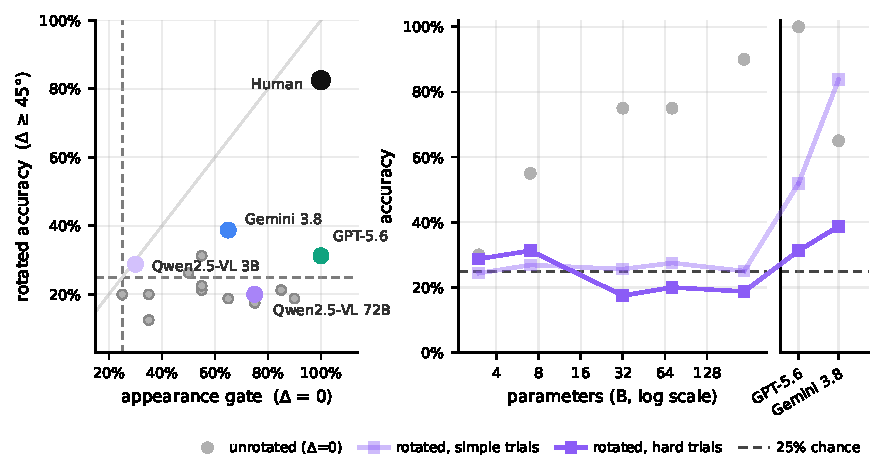
\includegraphics[width=\textwidth]{../../figures/fig1_gate_and_scaling.pdf}
  \caption{\textbf{Failure of allocentric invariance across models despite scaling.} (A) The appearance gate ($\Delta=0^\circ$) scales with model capability, reaching 100\% in GPT-5.6 Luna. (B) Allocentric performance ($\Delta \ge 45^\circ$) remains near chance (25\%) across all parameter scales (1B to 235B), revealing that scale buys a better visual gate, not a cognitive map.}
  \label{fig:cosyne}
\end{figure}

Frontier VLMs achieve ceiling or near-ceiling performance when the viewpoint is unchanged ($\Delta=0^\circ$, 100\% for GPT-5.6 Luna; Fig.~\ref{fig:cosyne}A), proving that their appearance gate successfully filters out changes in ground texture, lighting, and weather.
However, as soon as an observer rotation is introduced ($\Delta \ge 45^\circ$), performance drops precipitously to chance across all evaluated architectures (Fig.~\ref{fig:cosyne}B).
The error landscape exhibits a characteristic floor at $\Delta=135^\circ$ before recovering slightly at $\Delta=180^\circ$, consistent with 2D axis-inversion heuristics rather than genuine 3D allocentric transformation.
Critically, model accuracy does not scale with parameter count on rotated trials (flat scaling from 1B to 235B parameters), and test-time reasoning tokens produce no significant improvement over baseline prompts.

\section{Significance for Neural Systems}
Our results establish an empirical double dissociation between biological cognitive maps and artificial visual transformers.
Human observers exhibit allocentric competence through parahippocampal-entorhinal circuits that actively construct coordinate-free relational graphs.
In contrast, transformer-based vision architectures appear fundamentally constrained by their lack of explicit coordinate transformation mechanisms, path integration primitives, and recurrent attractor dynamics.
This work suggests that acquiring a biological-grade cognitive map will require dedicated neuro-inspired architectural inductive biases rather than compute-driven scaling alone.

\small
\bibliographystyle{plainnat}
\bibliography{refs}

\end{document}
